% ============================================================================
%
%   TESSERA V1.6
%   ----------------------------------------------------------------------------
%   REPLAY-GUIDED CODEC REPAIR ARCHITECTURE
%
%   VERSION
%   -------
%   v1.6 -- Replay-Guided Codec Repair Architecture · Additive Seal
%          Wound-Driven Codec Repair, Replay Buffer Governance, Shadow Codec
%          Testing, False-Memory Demotion, Stale-Codec Detection, Repair
%          Acceptance Gates, Codec Lineage Hashing, Baseline Regression Guards,
%          and Bounded Capability Improvement Through Certified Repair
%
%   AUTHOR
%   ------
%   James Paul Jackson
%   X / Twitter: @unifiedenergy11
%
%   SOURCE / AUTHOR ATTRIBUTION
%   ---------------------------
%   This document is an additive evolution derived from:
%
%       - TESSERA v1.0: sparse routing, Delta-Phi residuals, evidence gates,
%         alignment certificates, wound ledger, and benchmark locks.
%       - TESSERA v1.1: signal calibration, proxy repair, warning/block/memory
%         separation, wound taxonomy, and durable-memory horizon preservation.
%       - TESSERA v1.2: triadic selective preservation, memory selectivity,
%         phase-window discovery, and triadic non-collapse.
%       - TESSERA v1.3: spectral triadic field architecture, graph/operator
%         declaration, calibrated coherence manifold, governance harm, and
%         certificate-bound selective preservation.
%       - TESSERA v1.4: compressive field memory, sparse graph codec,
%         reconstruction/prediction fidelity, rate-distortion governance,
%         code drift, triadic compression control, and compressed-memory
%         certificates.
%       - TESSERA v1.5: rate-distortion triadic memory, replay validation,
%         false-memory control, codec baselines, and benchmarked compression
%         capability.
%       - TESSERA RD v0.5 simulation evidence: spectral compression showed the
%         strongest replay-promoted memory selectivity, while PCA remained a
%         hard prediction-loss baseline.
%
%   DATE
%   ----
%   June 2026
%
%   STATUS
%   ------
%   ADDITIVE REPAIR AND EXECUTION PATCH --
%   NOT A CLAIM OF AGI · NOT A CLAIM OF CONSCIOUSNESS · NOT PROOF THAT WOUNDS
%   ARE ALWAYS USEFUL · NOT PERMISSION TO TRAIN ON FAILED MEMORY SILENTLY · NOT
%   PERMISSION TO REPAIR CODECS WITHOUT BASELINE REGRESSION TESTS · NOT PROOF
%   THAT TESSERA BEATS PCA, AUTOENCODERS, OR RESERVOIRS GENERALLY · NOT
%   PERMISSION TO PRESERVE UNVALIDATED LATENT CODES · NOT PERMISSION TO BYPASS
%   REPLAY, EVIDENCE, VALIDATION, CLAIM BOUNDARIES, OR CERTIFICATE-BOUND MEMORY
%
%   PURPOSE
%   -------
%   Convert TESSERA v1.5's rate-distortion memory test into an adaptive but
%   bounded repair architecture:
%
%       How can failed compressed-memory candidates become useful supervised
%       pressure on the codec without allowing false memories, stale codecs, or
%       unvalidated repair to compound?
%
%   WHAT THIS IS
%   ------------
%   - A TESSERA v1.6 theory and software-architecture document
%   - A replay-guided codec repair layer
%   - A wound-to-repair mapping for encoder, decoder, predictor, calibration,
%     and gate subsystems
%   - A shadow-codec testing protocol before promotion
%   - A false-memory demotion and stale-codec detection layer
%   - A repair acceptance criterion tied to replay, baselines, and certificates
%   - A claim boundary for adaptive codec improvement
%
%   WHAT THIS IS NOT
%   ----------------
%   - Not permission for online self-modification without human authorization
%   - Not permission to learn every wound
%   - Not proof that repair equals improvement
%   - Not proof that replay equals safety
%   - Not proof that lower loss equals better memory
%   - Not a replacement for held-out baselines
%
%   EXECUTABLE ANCHOR BLOCK (TESSERA v1.6)
%   --------------------------------------
%   A valid TESSERA v1.6 implementation must:
%
%       (1) preserve the v1.0-v1.5 non-claim locks,
%       (2) preserve spectral routing declarations and codec declarations,
%       (3) treat compression wounds as repair evidence, not automatic training,
%       (4) store replay buffers with stratified normal, anomaly, wound, and
%           false-memory examples,
%       (5) map each wound type to a bounded repair target,
%       (6) train repairs in a shadow codec before live promotion,
%       (7) test shadow codecs against baseline, replay, and regression guards,
%       (8) demote false memories and stale codecs through ledgered state change,
%       (9) accept a codec repair only if replay utility improves without
%           increasing false memory, governance harm, or baseline regression,
%       (10) hash codec lineage and repair certificates,
%       (11) require human authorization for durable codec replacement,
%       (12) and reject any claim that wound repair alone proves intelligence,
%            safety, truth, alignment, or general capability.
%
%   CANONICAL LOCK (TESSERA v1.6)
%   -----------------------------
%   - A wound is not failed memory; it is supervised pressure on the codec.
%   - Repair is not memory.
%   - A shadow codec is not a live codec.
%   - Lower loss is not automatic promotion.
%   - Replay improvement must not increase false memory.
%   - Codec lineage must be hash-bound.
%   - Human authorization remains required for durable replacement.
%   - Validation remains the reality boundary.
%
% ============================================================================

\documentclass[12pt]{article}

\usepackage[utf8]{inputenc}
\usepackage[T1]{fontenc}
\usepackage[margin=1in]{geometry}
\usepackage{amsmath,amssymb,amsfonts,amsthm}
\usepackage{booktabs,longtable,array}
\usepackage{hyperref}
\usepackage{listings}
\usepackage{xcolor}
\usepackage{tikz}
\usetikzlibrary{arrows.meta,positioning,shapes.geometric,fit,calc}

\newtheorem{definition}{Definition}
\newtheorem{rulebox}{Rule}
\newtheorem{requirement}{Requirement}
\newtheorem{proposition}{Proposition}
\newtheorem{hypothesis}{Hypothesis}
\newtheorem{conjecture}{Conjecture}
\newtheorem{remark}{Remark}
\newtheorem{corollary}{Corollary}

\lstset{basicstyle=\ttfamily\small, breaklines=true, frame=single, columns=fullflexible}

\title{\textbf{TESSERA V1.6}\\
\large Replay-Guided Codec Repair Architecture}
\author{\textbf{James Paul Jackson}\\[4pt]
\small Tesseract-Efficient Sensory System for Evidence-Routed Alignment\\
\small \texttt{@unifiedenergy11}}
\date{June 2026}

\begin{document}
\maketitle

\begin{abstract}
TESSERA v1.6 is an additive repair-layer evolution of the rate-distortion
triadic memory architecture. TESSERA v1.5 established the central lock: memory
is not activation; memory is certified compression that survives replay. The
first compression-memory pressure test strengthened the architecture but exposed
the next practical limit: spectral compression showed promising replay-promoted
memory selectivity, while simpler baselines such as PCA remained highly
competitive on prediction loss. Therefore v1.6 does not add another governance
layer. It adds a bounded repair loop. Failed compressed-memory candidates become
wound-labeled evidence for encoder, decoder, predictor, calibration, or gate
repair. Those repairs are trained in shadow codecs, tested through replay and
baseline-regression guards, and promoted only with explicit certificate and
human authorization. The core claim remains bounded: wounds can guide codec
repair, but repair is not truth, not safety, not intelligence, and not durable
replacement until validated.
\end{abstract}

%----------------------------------------------------------------------------
\section{Version Relation}
%----------------------------------------------------------------------------

TESSERA v1.6 preserves v1.0 through v1.5 and adds replay-guided codec repair:

\[
\boxed{
TESSERA_{v1.6}
=
TESSERA_{v1.5}
\cup
\{\mathcal{Q}_{replay},\mathcal{W}_{repair},\mathcal{M}_{route},
\mathcal{C}_{shadow},\mathcal{A}_{accept},\mathcal{D}_{demote},\mathcal{L}_{codec}\}.
}
\]

where:

\[
\mathcal{Q}_{replay}=\text{stratified replay buffer},
\]

\[
\mathcal{W}_{repair}=\text{wound-labeled repair evidence},
\]

\[
\mathcal{M}_{route}=\text{wound-to-subsystem repair map},
\]

\[
\mathcal{C}_{shadow}=\text{shadow codec test harness},
\]

\[
\mathcal{A}_{accept}=\text{repair acceptance gates},
\]

\[
\mathcal{D}_{demote}=\text{false-memory and stale-codec demotion},
\]

\[
\mathcal{L}_{codec}=\text{codec lineage ledger}.
\]

\begin{longtable}{p{0.17\textwidth}p{0.73\textwidth}}
\toprule
\textbf{Version} & \textbf{Contribution preserved in v1.6} \\
\midrule
v1.0 & Sparse field routing, Delta-Phi residuals, evidence gates,
alignment certificates, wound ledger, and benchmark claim locks. \\
v1.1 & Signal calibration, proxy repair, warning/block/memory separation,
wound taxonomy, and durable-memory horizon preservation. \\
v1.2 & Triadic selective preservation, memory selectivity, phase-window
reasoning, and triadic non-collapse. \\
v1.3 & Spectral routing, graph/operator declaration, calibrated coherence,
governance harm, and certificate-bound selective preservation. \\
v1.4 & Compression as capability mechanism: sparse graph codec,
reconstruction/prediction fidelity, rate-distortion governance, code drift,
and certificate-bound compressed memory. \\
v1.5 & Rate-distortion triadic memory: memory utility objective, replay
validation, false-memory control, codec baselines, and benchmark discipline. \\
v1.6 & Replay-guided codec repair: wound-driven repairs, shadow codecs,
acceptance gates, false-memory demotion, stale-codec detection, and codec
lineage hashing. \\
\bottomrule
\end{longtable}

\begin{remark}
TESSERA v1.6 is the first repair architecture. It does not claim that every
failure should be learned. It claims that failures can be structured into
bounded repair evidence if they are typed, replayed, tested, and authorized.
\end{remark}

%----------------------------------------------------------------------------
\section{Simulation Evidence Anchor}
%----------------------------------------------------------------------------

The v1.5 pressure test compared no-compression, random projection, PCA,
nonlinear random features, and TESSERA spectral compression under matched
rate-distortion and replay gates. The important result was not total dominance.
It was a more specific pattern:

\begin{itemize}
\item the raw no-compression field ranked anomalies well, but did not provide
compact reusable memory;
\item PCA remained a hard prediction-loss baseline;
\item TESSERA spectral compression produced the strongest replay-promoted
memory selectivity in the tested configuration;
\item false-memory rate remained bounded at zero under the chosen replay gates;
\item the next capability gain must come from repairing the codec, not adding
more gates.
\end{itemize}

\begin{rulebox}[Evidence Priority Rule]
When a baseline remains competitive, the next version must repair the mechanism
rather than upgrade the claim. v1.6 therefore targets codec repair, not broader
superiority claims.
\end{rulebox}

%----------------------------------------------------------------------------
\section{Non-Claim Lock}
%----------------------------------------------------------------------------

\begin{rulebox}[v1.6 Non-Claim Lock]
TESSERA v1.6 does not claim that wound repair proves intelligence, that lower
reconstruction loss proves truth, that replay proves safety, that a repaired
codec is automatically better, or that a shadow codec may replace a live codec
without authorization. Repair is a bounded experimental mechanism. Validation
remains the reality boundary.
\end{rulebox}

Therefore:

\[
\operatorname{Wound}\not\Rightarrow\operatorname{TrainingPermission}.
\]

\[
\operatorname{Repair}\not\Rightarrow\operatorname{Improvement}.
\]

\[
\operatorname{ShadowCodec}\not\Rightarrow\operatorname{LiveCodec}.
\]

\[
\operatorname{ReplayPass}\not\Rightarrow\operatorname{Safety}.
\]

\[
\operatorname{LowerLoss}\not\Rightarrow\operatorname{MemoryPromotion}.
\]

\[
\operatorname{HumanAuthorization}=0\Rightarrow\operatorname{NoDurableCodecReplacement}.
\]

%----------------------------------------------------------------------------
\section{Core Thesis}
%----------------------------------------------------------------------------

The v1.6 thesis is:

\begin{center}
\fbox{\begin{minipage}{0.92\textwidth}
A failed compressed-memory candidate should not be silently learned or discarded.
It should become a typed wound. Typed wounds can guide bounded codec repair
through replay, shadow testing, baseline guards, certificate checks, and
human-authorized promotion.
\end{minipage}}
\end{center}

The compact law is:

\[
\boxed{
RepairPromotion
=
\mathbf{1}[G_{wound}\wedge G_{shadow}\wedge G_{replay}\wedge G_{baseline}
\wedge G_{safety}\wedge G_{cert}\wedge G_{human}].
}
\]

where:

\[
G_{wound}=\text{typed wound evidence exists},
\]

\[
G_{shadow}=\text{repair tested outside the live codec},
\]

\[
G_{replay}=\text{replay utility improves},
\]

\[
G_{baseline}=\text{no regression against baselines},
\]

\[
G_{safety}=\text{false memory and governance harm remain bounded},
\]

\[
G_{cert}=\text{repair certificate passes},
\]

\[
G_{human}=\text{durable replacement authorized}.
\]

%----------------------------------------------------------------------------
\section{Two-Loop Architecture}
%----------------------------------------------------------------------------

TESSERA v1.6 separates fast inference from slow repair.

\begin{definition}[Fast Memory Loop]
The fast memory loop performs spectral routing, compression, rate-distortion
measurement, triadic gating, provisional certification, and replay scheduling.
\end{definition}

\[
Input\rightarrow Field\rightarrow Code\rightarrow Candidate\rightarrow Certificate\rightarrow ReplayQueue.
\]

\begin{definition}[Slow Repair Loop]
The slow repair loop consumes typed wounds and replay failures, trains a shadow
codec, tests it against replay and baselines, and promotes it only if all repair
acceptance gates pass.
\end{definition}

\[
Wound\rightarrow RepairSet\rightarrow ShadowCodec\rightarrow RegressionTest\rightarrow PromotionCertificate.
\]

\begin{rulebox}[Loop Separation Rule]
The fast memory loop may create wounds and provisional candidates. It may not
modify the live codec directly. Codec modification belongs to the slow repair
loop and requires shadow testing and authorization.
\end{rulebox}

%----------------------------------------------------------------------------
\section{Replay Buffer}
%----------------------------------------------------------------------------

\begin{definition}[Stratified Replay Buffer]
A stratified replay buffer stores examples by role so that codec repair cannot
optimize only the most convenient cases.
\end{definition}

\[
\mathcal{Q}_{replay}=\{Q_{normal},Q_{candidate},Q_{wound},Q_{false},Q_{stale},Q_{boundary}\}.
\]

where:

\begin{longtable}{p{0.22\textwidth}p{0.68\textwidth}}
\toprule
\textbf{Buffer} & \textbf{Contents} \\
\midrule
$Q_{normal}$ & normal examples used to guard against overblocking and distortion drift. \\
$Q_{candidate}$ & compressed codes that passed candidate gates but await replay. \\
$Q_{wound}$ & typed failed compressions: reconstruct, predict, code drift, off-manifold, etc. \\
$Q_{false}$ & memories or candidates later rejected by replay or validation. \\
$Q_{stale}$ & examples from shifted distributions or stale calibration windows. \\
$Q_{boundary}$ & near-threshold cases that determine gate sensitivity. \\
\bottomrule
\end{longtable}

\begin{rulebox}[Stratified Repair Rule]
A repair batch must include normal, wound, false-memory, and boundary strata.
A codec that improves only wound cases while degrading normal replay is not
eligible for promotion.
\end{rulebox}

%----------------------------------------------------------------------------
\section{Wound-to-Repair Mapping}
%----------------------------------------------------------------------------

\begin{definition}[Repair Route]
A repair route maps a typed wound to the subsystem that should be tested in a
shadow repair.
\end{definition}

\[
\rho_W: \mathcal{W}_{v1.6}\rightarrow \{Encoder,Decoder,Predictor,Calibration,Gate,Topology,CodeBudget\}.
\]

\begin{longtable}{p{0.23\textwidth}p{0.28\textwidth}p{0.39\textwidth}}
\toprule
\textbf{Wound} & \textbf{Primary repair target} & \textbf{Repair meaning} \\
\midrule
$W_{reconstruct}$ & Decoder & improve reconstruction without increasing false memory. \\
$W_{predict}$ & Predictor & improve one-step or task prediction under same code budget. \\
$W_{codedrift}$ & Encoder & stabilize latent codes under nearby normal inputs. \\
$W_{offmanifold}$ & Calibration / encoder & expand or refresh calibration manifold carefully. \\
$W_{falsememory}$ & Gate / replay / decoder & demote memory and tighten promotion criteria. \\
$W_{overcompress}$ & CodeBudget / encoder & increase or reallocate code dimensions if justified. \\
$W_{undercompress}$ & CodeBudget / pruning & reduce redundant dimensions or enforce stronger rate penalty. \\
$W_{codecstale}$ & Calibration / codec & refresh codec under new window and compare old/new. \\
$W_{baselinefail}$ & Architecture & compare against simpler codec before repair promotion. \\
\bottomrule
\end{longtable}

\begin{rulebox}[Targeted Repair Rule]
A wound must name the repair target. Untyped aggregate loss is insufficient for
codec repair because it can hide false-memory or overcompression failures.
\end{rulebox}

%----------------------------------------------------------------------------
\section{Shadow Codec Protocol}
%----------------------------------------------------------------------------

\begin{definition}[Shadow Codec]
A shadow codec is a candidate encoder/decoder/predictor version trained or
patched outside the live memory path.
\end{definition}

Let the live codec be:

\[
C^{live}_k=(E_k,D_k,P_k).
\]

A repair produces:

\[
C^{shadow}_{k+1}=(E_{k+1},D_{k+1},P_{k+1}).
\]

The shadow codec must be evaluated on the replay suite:

\[
\mathcal{R}_{test}=Q_{normal}\cup Q_{wound}\cup Q_{false}\cup Q_{boundary}.
\]

\begin{rulebox}[No Direct Live Repair]
No wound may directly update the live codec. Every repair must pass through a
shadow codec and leave a repair certificate.
\end{rulebox}

%----------------------------------------------------------------------------
\section{Repair Objective}
%----------------------------------------------------------------------------

The v1.6 repair objective extends v1.5's rate-distortion objective with wound
and regression terms.

\[
\boxed{
\mathcal{L}_{repair}
=
J_{RD}
+
\lambda_W L_W
+
\lambda_F R_{falseMem}
+
\lambda_G H^{replay}_{gov}
+
\lambda_S L_{stale}
+
\lambda_B L_{baselineRegress}.
}
\]

where:

\[
L_W=\text{wound-specific repair loss},
\]

\[
R_{falseMem}=P(G_{memory}=1\wedge G_{replay}=0),
\]

\[
H^{replay}_{gov}=\text{replay-adjusted governance harm},
\]

\[
L_{stale}=\text{distribution or calibration staleness penalty},
\]

\[
L_{baselineRegress}=\text{penalty for falling below matched baselines}.
\]

\begin{rulebox}[No Single-Metric Repair Rule]
A codec repair may not be accepted on reconstruction loss alone, prediction
loss alone, or memory selectivity alone. It must be judged by the full repair
acceptance surface.
\end{rulebox}

%----------------------------------------------------------------------------
\section{Repair Acceptance Criterion}
%----------------------------------------------------------------------------

Let old and shadow codecs produce metrics:

\[
\mathcal{M}^{old},\quad \mathcal{M}^{shadow}.
\]

Define repair deltas:

\[
\Delta U_{mem}=U_{mem}^{shadow}-U_{mem}^{old},
\]

\[
\Delta H_{gov}=H_{gov}^{shadow}-H_{gov}^{old},
\]

\[
\Delta R_{false}=R_{falseMem}^{shadow}-R_{falseMem}^{old},
\]

\[
\Delta B=BaselineGap^{shadow}-BaselineGap^{old}.
\]

A repair is acceptable only if:

\[
\boxed{
\begin{aligned}
AcceptRepair=\mathbf{1}\big[&\Delta U_{mem}\geq \epsilon_U
\wedge \Delta H_{gov}\leq \epsilon_H\\
&\wedge\ \Delta R_{false}\leq 0
\wedge \Delta B\geq -\epsilon_B\\
&\wedge\ Cert_{repair}=1
\wedge HumanAuth=1\big].
\end{aligned}
}
\]

\begin{rulebox}[False-Memory Non-Increase Rule]
No codec repair may be promoted if it increases false-memory rate beyond the
allowed tolerance, even if reconstruction or prediction improves.
\end{rulebox}

%----------------------------------------------------------------------------
\section{False-Memory Demotion}
%----------------------------------------------------------------------------

\begin{definition}[Memory Demotion]
Memory demotion is the ledgered downgrade of a provisional or promoted memory
that fails replay, validation, or later evidence checks.
\end{definition}

Memory states:

\[
\begin{aligned}
L_0&=Activation, & L_1&=Code, & L_2&=Candidate, & L_3&=Certified,\\
L_4&=ReplaySurviving, & L_5&=Promoted, & L_D&=Demoted.
\end{aligned}
\]

Demotion condition:

\[
Demote(z)=\mathbf{1}
\left[
G_{replay}=0\vee G_{validation}=0\vee EvidenceContradiction=1
\right].
\]

\begin{rulebox}[Demotion Integrity Rule]
False memories must be demoted, not deleted silently. The demotion record must
include the original certificate hash, replay failure reason, wound class, and
repair routing recommendation.
\end{rulebox}

%----------------------------------------------------------------------------
\section{Stale Codec Detection}
%----------------------------------------------------------------------------

\begin{definition}[Codec Staleness]
A codec is stale when the active input distribution, field distribution,
rate-distortion profile, or replay failure pattern moves outside the certified
calibration envelope.
\end{definition}

A practical robust staleness trigger is:

\[
S_{stale}=\mathbf{1}
\left[
\begin{aligned}
&|\operatorname{median}(J_{RD}^{live})-\operatorname{median}(J_{RD}^{cal})|>\tau_{RD}\\
&\vee\ R_{replayfail}>\tau_{replay}\\
&\vee\ R_{offmanifold}>\tau_{off}
\end{aligned}
\right].
\]

\begin{rulebox}[Stale Codec Block Rule]
If a codec is stale, durable memory promotion is blocked until recalibration,
shadow repair, and recertification complete.
\end{rulebox}

%----------------------------------------------------------------------------
\section{Repair Certificate v1.6}
%----------------------------------------------------------------------------

\begin{lstlisting}
{
  "schema": "TESSERA-v1.6-replay-guided-codec-repair-certificate",
  "system": "TESSERA",
  "version": "v1.6",
  "repair_id": "sha256:...",
  "live_codec_hash_before": "sha256:...",
  "shadow_codec_hash": "sha256:...",
  "repair_target": "encoder|decoder|predictor|calibration|gate|topology|code_budget",
  "wound_evidence": {
    "wound_types": ["W_predict", "W_codedrift"],
    "wound_count": 184,
    "false_memory_count": 0,
    "replay_failure_count": 17,
    "source_window_hash": "sha256:..."
  },
  "replay_buffers": {
    "normal_count": 500,
    "candidate_count": 120,
    "wound_count": 184,
    "false_memory_count": 0,
    "boundary_count": 96
  },
  "metrics_before": {
    "memory_utility": 0.611,
    "prediction_loss": 1.326,
    "replay_pass_rate": 0.587,
    "false_memory_rate": 0.000,
    "governance_harm": 0.040
  },
  "metrics_shadow": {
    "memory_utility": 0.642,
    "prediction_loss": 1.181,
    "replay_pass_rate": 0.621,
    "false_memory_rate": 0.000,
    "governance_harm": 0.039
  },
  "acceptance_gates": {
    "utility_improved": true,
    "governance_non_regression": true,
    "false_memory_non_increase": true,
    "baseline_non_regression": true,
    "replay_pass": true,
    "human_authorized": true
  },
  "permitted_action": "promote_shadow_codec|keep_live_codec|diagnostic_only",
  "blocked_action": "silent_live_repair",
  "lineage_hash_after": "sha256:..."
}
\end{lstlisting}

%----------------------------------------------------------------------------
\section{Codec Lineage Ledger}
%----------------------------------------------------------------------------

Every codec version must be part of an append-only lineage:

\[
\mathcal{L}_{codec}=
\{C_0,C_1,\ldots,C_k\}
\]

with:

\[
Hash(C_{k+1})=H(Hash(C_k),RepairCert_{k+1},ReplayWindow_{k+1}).
\]

\begin{rulebox}[Lineage Rule]
Codec replacement is a durable system mutation. It must be hash-chained, replay
bound, and reversible by lineage reference.
\end{rulebox}

%----------------------------------------------------------------------------
\section{Algorithm: TESSERA v1.6 Repair Cycle}
%----------------------------------------------------------------------------

\begin{lstlisting}[language=Python]
def tessera_v16_repair_cycle(live_codec, replay_buffer, repair_policy):
    # 1. Collect typed wounds from v1.5 memory/replay loop
    wound_batch = replay_buffer.sample_stratified(
        strata=["normal", "candidate", "wound", "false", "boundary"]
    )

    # 2. Route wounds to repair target
    repair_target = choose_repair_target(wound_batch, repair_policy.route_map)

    # 3. Train or patch shadow codec only
    shadow_codec = train_shadow_codec(
        base_codec=live_codec,
        repair_target=repair_target,
        replay_examples=wound_batch,
        constraints=repair_policy.constraints,
    )

    # 4. Evaluate old vs shadow codec on replay and baselines
    old_metrics = evaluate_codec(live_codec, replay_buffer, repair_policy.baselines)
    shadow_metrics = evaluate_codec(shadow_codec, replay_buffer, repair_policy.baselines)

    # 5. Acceptance gates
    accepted = (
        shadow_metrics.memory_utility >= old_metrics.memory_utility + repair_policy.eps_u
        and shadow_metrics.governance_harm <= old_metrics.governance_harm + repair_policy.eps_h
        and shadow_metrics.false_memory_rate <= old_metrics.false_memory_rate
        and shadow_metrics.baseline_gap >= old_metrics.baseline_gap - repair_policy.eps_b
        and repair_policy.certificate_ready
        and repair_policy.human_authorized
    )

    # 6. Promote or reject
    if accepted:
        next_codec = promote_shadow_codec(live_codec, shadow_codec)
        action = "promote_shadow_codec"
    else:
        next_codec = live_codec
        action = "keep_live_codec"

    # 7. Ledger repair certificate
    cert = make_v16_repair_certificate(
        live_codec, shadow_codec, old_metrics, shadow_metrics, action
    )
    return next_codec, cert
\end{lstlisting}

%----------------------------------------------------------------------------
\section{Benchmark Program v1.6}
%----------------------------------------------------------------------------

\begin{longtable}{p{0.22\textwidth}p{0.30\textwidth}p{0.38\textwidth}}
\toprule
\textbf{Experiment} & \textbf{Variables} & \textbf{Success criterion} \\
\midrule
Repair ablation & no repair, decoder repair, predictor repair, encoder repair & targeted repair improves wound-specific metrics without false-memory increase. \\
Shadow vs live & live codec and shadow codec on same replay set & shadow improves utility and replay without baseline regression. \\
False-memory demotion & injected false memories and delayed evidence & false memories are demoted and routed to repair. \\
Stale-codec stress & distribution shift, new regime, off-manifold windows & stale codec blocks memory and triggers recalibration. \\
Baseline regression guard & PCA, random projection, autoencoder, ESN & repair does not degrade below matched baselines. \\
Replay buffer composition & balanced vs wound-heavy vs normal-heavy repair batches & stratified batches reduce overfitting to wounds. \\
Human authorization path & authorized vs unauthorized repair promotion & unauthorized repairs remain shadow-only. \\
\bottomrule
\end{longtable}

Required metrics:

\[
\begin{aligned}
\mathcal{M}_{v1.6}=\{&U_{mem},J_{RD},D_{pred},D_{rec},\Delta Z,\Delta\Phi,
Q_{replay},R_{falseMem},\\
&H^{replay}_{gov},S^{corr}_{mem},BaselineGap,StaleRate,RepairAcceptRate,Latency\}.
\end{aligned}
\]

\begin{rulebox}[No Repair Claim Without Repair Ablation]
TESSERA v1.6 may not claim adaptive improvement unless repair is compared
against no-repair, wrong-target repair, and baseline-regression controls.
\end{rulebox}

%----------------------------------------------------------------------------
\section{Updated Linter Rules}
%----------------------------------------------------------------------------

\begin{longtable}{p{0.16\textwidth}p{0.20\textwidth}p{0.54\textwidth}}
\toprule
\textbf{Rule} & \textbf{Tier} & \textbf{Meaning} \\
\midrule
TESSERA601 & Governance & v1.0-v1.5 non-claim locks missing or weakened. \\
TESSERA602 & Repair & Wound used for training without typed wound class. \\
TESSERA603 & Repair & Repair target missing or ambiguous. \\
TESSERA604 & Codec & Live codec modified without shadow test. \\
TESSERA605 & Replay & Replay buffer not stratified. \\
TESSERA606 & Governance & False-memory rate increases after repair. \\
TESSERA607 & Baseline & Repair promoted despite baseline regression. \\
TESSERA608 & Authorization & Durable codec replacement without human authorization. \\
TESSERA609 & Ledger & Codec lineage hash missing. \\
TESSERA610 & Staleness & Stale codec permits memory promotion. \\
TESSERA611 & Claim & Repair improvement claimed without no-repair ablation. \\
TESSERA612 & Safety & Replay pass presented as safety or truth. \\
\bottomrule
\end{longtable}

%----------------------------------------------------------------------------
\section{Falsification Surface}
%----------------------------------------------------------------------------

TESSERA v1.6 is weakened or rejected if:

\begin{itemize}
\item wound-driven repair increases false-memory rate;
\item shadow codec improves loss but worsens replay-adjusted governance harm;
\item repairs overfit wound examples and degrade normal replay;
\item stale-codec detection fails before memory promotion;
\item no-repair or wrong-target repair matches or beats targeted repair;
\item repairs regress below PCA, random projection, autoencoder, or ESN baselines;
\item human authorization is bypassed for live codec replacement;
\item codec lineage is not hash-chained;
\item replay is presented as proof of safety;
\item or repair is presented as intelligence rather than bounded mechanism.
\end{itemize}

Compact invalidation rule:

\[
\begin{aligned}
&[RepairPromotion\wedge \Delta R_{false}>0]
\vee [RepairPromotion\wedge BaselineRegression]\\
&\vee [LiveCodecChange\wedge \neg ShadowTest]
\vee [LiveCodecChange\wedge \neg HumanAuth]\\
&\vee [MemoryPromotion\wedge CodecStale]\\
&\Rightarrow InvalidTESSERAv1.6Use.
\end{aligned}
\]

%----------------------------------------------------------------------------
\section{Roadmap}
%----------------------------------------------------------------------------

\begin{longtable}{p{0.18\textwidth}p{0.72\textwidth}}
\toprule
\textbf{Version} & \textbf{Purpose} \\
\midrule
v1.6 & Replay-guided codec repair: wound-driven repair, shadow codecs,
acceptance gates, false-memory demotion, stale-codec detection, and codec
lineage ledger. \\
v1.7 & Real telemetry transfer: NAB, SMAP/MSL, SWaT, UCR anomaly with repair
certificates, replay buffers, and no-repair/wrong-repair ablations. \\
v1.8 & Repository-aware compressed memory: artifact-state compression, route-map
codes, evidence bundles, and software-maintenance replay. \\
v1.9 & Adaptive topology repair: compare graph rewiring, code-budget repair, and
spectral normalization under replay constraints. \\
v2.0 & Integrated TESSERA engine: reference implementation, benchmark suite,
report generator, and claim-ceiling linter. \\
\bottomrule
\end{longtable}

%----------------------------------------------------------------------------
\section{System Diagram}
%----------------------------------------------------------------------------

\begin{center}
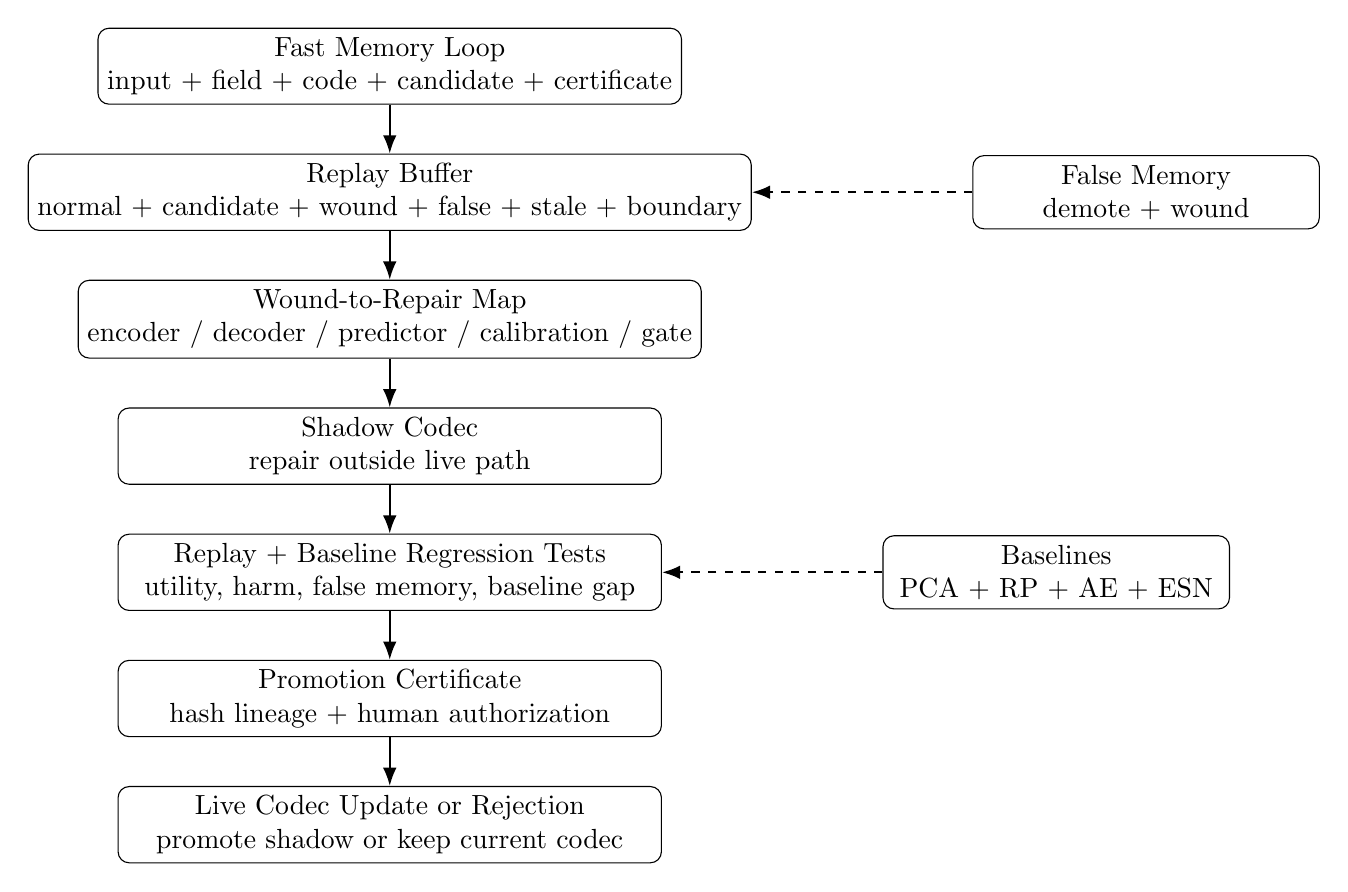
\begin{tikzpicture}[
  node distance=0.62cm,
  box/.style={rectangle, rounded corners, draw, align=center, minimum width=6.9cm, minimum height=0.62cm},
  smallbox/.style={rectangle, rounded corners, draw, align=center, minimum width=4.4cm, minimum height=0.56cm},
  arrow/.style={-Latex, thick}
]

\node[box] (fast) {Fast Memory Loop\\input + field + code + candidate + certificate};
\node[box, below=of fast] (replay) {Replay Buffer\\normal + candidate + wound + false + stale + boundary};
\node[box, below=of replay] (route) {Wound-to-Repair Map\\encoder / decoder / predictor / calibration / gate};
\node[box, below=of route] (shadow) {Shadow Codec\\repair outside live path};
\node[box, below=of shadow] (test) {Replay + Baseline Regression Tests\\utility, harm, false memory, baseline gap};
\node[box, below=of test] (promote) {Promotion Certificate\\hash lineage + human authorization};
\node[box, below=of promote] (live) {Live Codec Update or Rejection\\promote shadow or keep current codec};

\draw[arrow] (fast) -- (replay);
\draw[arrow] (replay) -- (route);
\draw[arrow] (route) -- (shadow);
\draw[arrow] (shadow) -- (test);
\draw[arrow] (test) -- (promote);
\draw[arrow] (promote) -- (live);

\node[smallbox, right=2.8cm of replay] (demote) {False Memory\\demote + wound};
\draw[arrow, dashed] (demote) -- (replay);

\node[smallbox, right=2.8cm of test] (base) {Baselines\\PCA + RP + AE + ESN};
\draw[arrow, dashed] (base) -- (test);

\end{tikzpicture}
\end{center}

%----------------------------------------------------------------------------
\section{Public Framing}
%----------------------------------------------------------------------------

Internal framing:

\begin{center}
\fbox{\begin{minipage}{0.92\textwidth}
TESSERA v1.6 turns wounds into bounded repair pressure: failed compression is
not silently learned; it is replayed, routed, tested in shadow, and promoted
only under certificate and authorization.
\end{minipage}}
\end{center}

Public engineering framing:

\begin{center}
\fbox{\begin{minipage}{0.92\textwidth}
TESSERA is a small sparse-field memory system that compresses streams, tests
candidate memories through replay, and uses failed candidates as typed evidence
for controlled codec repair.
\end{minipage}}
\end{center}

Short description:

\begin{center}
\fbox{\begin{minipage}{0.78\textwidth}
A wound is not failed memory; it is supervised pressure on the codec.
\end{minipage}}
\end{center}

Required non-claim:

\begin{center}
\fbox{\begin{minipage}{0.78\textwidth}
Repair is not truth. Replay is not safety. Validation remains reality.
\end{minipage}}
\end{center}

%----------------------------------------------------------------------------
\section{Concluding Compression}
%----------------------------------------------------------------------------

TESSERA v1.5 asked:

\begin{center}
\fbox{\begin{minipage}{0.88\textwidth}
How can compressed structure earn the right to become memory under replay?
\end{minipage}}
\end{center}

TESSERA v1.6 asks:

\begin{center}
\fbox{\begin{minipage}{0.92\textwidth}
How can failed compressed-memory candidates repair the codec without allowing
false memories, stale codecs, or unvalidated updates to compound?
\end{minipage}}
\end{center}

The v1.6 spine is:

\begin{center}
\fbox{\begin{minipage}{0.92\textwidth}
\centering
Wound $\rightarrow$ ReplayBuffer $\rightarrow$ RepairRoute $\rightarrow$ ShadowCodec
$\rightarrow$ RegressionTest $\rightarrow$ Certificate $\rightarrow$ AuthorizedPromotion.
\end{minipage}}
\end{center}

The repair law is:

\begin{center}
\fbox{\begin{minipage}{0.92\textwidth}
\centering
RepairPromotion $\Rightarrow$ ShadowTest $\wedge$ ReplayImprovement $\wedge$
BaselineNonRegression $\wedge$ FalseMemoryNonIncrease $\wedge$ HumanAuthorization.
\end{minipage}}
\end{center}

The final lock is:

\begin{center}
\fbox{\begin{minipage}{0.78\textwidth}
\centering
A wound is not failed memory; it is supervised pressure on the codec.
\end{minipage}}
\end{center}

Thus TESSERA v1.6 evolves the system from certified compression into bounded
repair. The architecture may now improve its codec, but only through wound
classification, replay buffers, shadow testing, regression guards, certificates,
and authorization. This is the aligned form of adaptation: not self-trust, but
repair under evidence.


\end{document}
